\documentclass[12pt]{article}
\usepackage{amsmath}
\usepackage[english]{babel}
\usepackage[utf8x]{inputenc}
\usepackage[T1]{fontenc}
\usepackage{url}
\usepackage{scribe}
\usepackage{listings}
\usepackage{mathtools}
\usepackage{listings}
\usepackage{tikz}
\usepackage{xcolor}

\lstdefinestyle{mystyle}{
    backgroundcolor=\color{backcolour},   
    commentstyle=\color{codegreen},
    keywordstyle=\color{magenta},
    numberstyle=\tiny\color{codegray},
    stringstyle=\color{codepurple},
    basicstyle=\ttfamily\footnotesize,
    breakatwhitespace=false,         
    breaklines=true,                 
    captionpos=b,                    
    keepspaces=true,                 
    numbers=left,                    
    numbersep=5pt,                  
    showspaces=false,                
    showstringspaces=false,
    showtabs=false,                  
    tabsize=2
}

\tikzstyle{data} = [circle, minimum size = 3 cm,text centered, draw=black, thick, fill=red!30, text=white]
\tikzstyle{model} = [rectangle, minimum width=3cm, minimum height=3cm, text centered, draw=black, fill=orange!30]
\tikzstyle{arrow} = [thick,->,>=stealth]
\tikzstyle{outp} = [rectangle, rounded corners, minimum width=3cm, minimum height=3cm,text centered, draw=black, fill=green!30]

\Scribe{Group 5,6}
\Lecturer{Abir De}
\LectureNumber{15}
\LectureDate{15 March 2023}
\LectureTitle{Kernel Methods}

\lstset{style=mystyle}

\begin{document}
	\MakeScribeTop

 
% Here's a typical LP in standard/equational form, with an equation number on one of the constraints.
% \begin{gather}
%     \min \quad c^\top x                       \nonumber\\
%     \begin{aligned}
%         \text{s.t.} \quad   Ax &= b           \nonumber\\
%                              x &\geq 0       \label{eqn:nonnegative}
%     \end{aligned}
% \end{gather}

% \noindent Here's a reference to the~\eqref{eqn:nonnegative} nonnegativity constraint.  Some more LPs:


% More generically:
% \[
%     A = \begin{bmatrix}
%             \vrule & \vrule & & \vrule\\
%             A_{1} & A_{2} & \cdots & A_{n} \\
%             \vrule & \vrule & & \vrule
%         \end{bmatrix}
%       = \begin{bmatrix}
%             \text{---} & a_1 & \text{---} \\
%             \text{---} & a_1 & \text{---} \\
%                        & \vdots &  \\
%             \text{---} & a_n & \text{---} 
%         \end{bmatrix}
% \]


% Here's some more random typesetting: 
% \begin{itemize}
% \item ``PTIME vs. NP, where the former means time $\poly(n)$'';
% \item $\wt{O}(f(x)) \text{ is } f(x) \cdot \polylog(f(x))$;
% \item $\displaystyle 
%         g(x) = \begin{cases}
%                    \sin(2\theta) & \text{if $\theta \leq \pi$,}\\
%                    \max\{\cos^2\theta, \tfrac13\} & \text{if $\theta > \pi$.}
%                \end{cases}
%       $
% \end{itemize}
% Please don't write $max(A)$ when you mean $\max(A)$, or $log(n)$ when you mean $\log(n)$, or "quotes" when you mean ``quotes''.

% \

% More equations:

% $\max \Big\{ \sum_{i \in Observations} \Big( y_i - \sum_{j \in Candidates} \beta_j x_{i,j} \Big) ^2 \Big\}$

% $\max\Bigg\{ \sum_{i \in Observations} \Big| y_i - \sum_{j \in Candidates} \beta_j x_{i,j} \Big| \Bigg\}$

% A theorem and a proof:
% \begin{theorem} $(a+b)^2 = a^2 + 2ab + b^2$.
% \end{theorem}
% \begin{proof}
% Let for the reader.
% \end{proof}

% \bigskip

% Here's what to do if your proof ends on an equation:
% \begin{proof}
% It's easy:
% \[
%     (a+b)^2 = (a+b)(a+b) = (a+b)a + (a+b)b = a^2 + ba + ab + b^2 = a^2 + 2ab + b^2 \qedhere
% \]
% \end{proof}

% And a lemma without proof:
% \begin{lemma}
% Suppose numbers exist, then $(a+b)^2 = a^2 + 2ab + b^2$.
% \end{lemma}

% You can do a few others:
% \begin{example}
% Suppose numbers exist, then $(a+b)^2 = a^2 + 2ab + b^2$.
% \end{example}
% \begin{conjecture}
% Suppose numbers exist, then $(a+b)^2 = a^2 + 2ab + b^2$.
% \end{conjecture}
% \begin{definition}
%d-out stuff in the \LaTeX~here.

% \

% My farourive Optimization books are \cite{bertsimas1997introduction} \cite{boyd2004convex} \cite{wolsey2014integer}. You should add bibliographical notes in the \textbf{BibTex}: \textit{mybib.bib} file. Its good to grab these notes from Google scholar citations.

% %%%%%%%%%%% If you don't have citations then comment the lines below:
% %

In the previous lecture, we have had an introduction on the basics of Kernel and its properties. Then we went on to see some populars Kernels in the tutorial session also. In this lecture we go on to build up on Kernels and solve SVM problems through Kernel Methods.

\section{Introduction}

 Let us take a short recap of what we studied in the last lecture and then continue on to the todays content for a better flow. \\
 Before we understand Kernels, we need to understand the inner product and its propertise in a precise manner.
\subsection{Inner Product Space}

An inner product space over reals is a vector space $\mathcal{V}$ and an inner product, which is a mapping
\begin{center}
    $\langle\cdot,\cdot\rangle:\mathcal{V}\times\mathcal{V}\to\mathcal{\boldsymbol{R}}$
\end{center}
Following are the properties of inner product $\forall x,y,z\in \mathcal{V}$ and $a,b \in \mathcal{\boldsymbol{R}}$:-\\
\begin{itemize}
    \item Symmetry: $\langle x,y\rangle = \langle y,x \rangle$
    \item Linearity: $\langle ax+by,z \rangle = a\langle x,z\rangle + b\langle y,z \rangle $
    \item Positive-definiteness: $\langle x,x \rangle\geq 0$ and $\langle x,x \rangle=0 \iff x=0$
\end{itemize}

\subsection{Kernel}
The kernel by definition avoids the explicit mapping that is needed to get linear learning algorithms to learn a nonlinear function or decision boundary.\\

For all $ x $ and $x’$ in the input space $ \Phi $ certain functions $ K(x,x’) $ can be expressed as an inner product in another space $ \Psi $. The function \\
\begin{center}
    $ K: \Phi  \times \Phi \rightarrow \mathbb{R}$
\end{center}
$\forall x,x' \in \mathcal{X}$, 
\[K(x,x') = \langle \phi(x), \phi(x') \rangle_{\mathcal{}}\]

The Gram matrix is then defined as $ G_{i,j} = K(x_{i},x_{j}) $.\\
The two necessary condition for a kernel are: \\
\begin{itemize}
    \item Symmetric: $ K(x_{i}, x_{j}) = K(x_{j}, x_{i}) $
    \item Positive Semi Definite : $G_{i,j} >= 0$
\end{itemize} 

From the above understanding we can confirm that for a set of N data points there exist N Kernel Mappings.

\section{SVM Objective Function}

For the SVM mechanism we had already learnt the following objective function formulation: \\
\begin{equation}
    \label{loss_function}
    \underset{w}{min} \; \; l (\{w^{T}\phi(x_{i})\}_{i \in D}, \{y_{i}\}_{i \in D} ) + \lambda R(||w||)
\end{equation}
where $l : \mathbb{R}^{|D|} \rightarrow \mathbb{R}$ is an arbitrary function and $R : \mathbb{R}_{+} \rightarrow \mathbb{R}$ is a monotonically non-decreasing Regularization function.\\

We found out the optimal $\omega$ as:\\
\[w* = \sum_{i=1}^{|D|} \alpha_{i} \phi(x_{i})\]
Form of f is 
\begin{align*}
    f(x) &= {w^{*}}^{T}\phi(x_{i})  \\
        &= \sum_{i = 1}^{|D|} \alpha_{i} \phi^{T}(x_{i}) \phi(x)
\end{align*}
Here $\phi^{T}(x_{i}) \phi(x)$ is like a similarity measure
If $\phi(\cdot)$ is $\infty$-dimensional, we can write it as 
\[ f(x) =  \sum_{i = 1}^{|D|} \alpha_{i} \sum_{j=0}^{\infty} \phi(x_{i})[j] \phi(x)[j]\]
Thus, if $\phi(\cdot)$ is $\infty$-dimensional, it is very high computational task to compute $ {w^{*}}^{T}\phi(x_{i}) $ as $w$ as it has the same 
dimension as $\phi$. So, we try to represent the objective function in functional form or through the kernel formulation so that we would not have to do such computations.
 


\section{Kernel Formualation}

Now as in the last topic, we got stuck in the case when $\omega$ and $\phi(x_{i})$ are of infinite dimension, it gets impossible to find these vectors.\\
Hence here we try to formulate the objective function with the use of Kernels that we studied earlier.

Writing $w = \sum_{j=1}^{|D|} \alpha_{j} \phi(x_j)$,\\
we have that for all i
\[\langle w, \phi(x_{i})\rangle = \langle \sum_{j=1}^{|D|} \alpha_{j} \phi(x_j),\phi(x_{i}\rangle = \sum_{j = 1}^{|D|} \alpha_j \langle \phi(x_j), \phi(x_i)\rangle .\]
Similarly,
\[ ||w||^{2}  = \langle \sum_{j=1}^{|D|} \alpha_{j} \phi(x_j), \sum_{j=1}^{|D|} \alpha_{j} \phi(x_j) \rangle =  \sum_{i,j = 1}^{|D|} \alpha_i \alpha_j \langle \phi(x_i), \phi(x_j)\rangle .\]

Let $K(x,x') = \langle \phi(x), \phi(x') \rangle$ be a function that implements the kernel function
with respect to the feature space.
Hence, instead of solving Equation \ref{loss_function}, we can solve the equivalent problem
\begin{equation}
\underset{\alpha \in \mathbb{R}^{|D|}}{min}  l (\{\sum_{j=1}^{|D|}\alpha_j K(x_j,x_{i})\}_{i \in D}, \{y_{i}\}_{i \in D} ) + \lambda R(\sqrt{\sum_{i,j =1}^{|D|} \alpha_i \alpha_j K(x_{j},x_{i})})   
\end{equation}
\section{Probability Gaussian Process}

Now that we have gained enough knowledge on Kernels, its properties and also its formulation. Here we take our discussion further on another application of kernels in the context of Gaussian Processes and how to deal with smaller training sets to still give fair results.

Now we already know the objective function as

\[w^{\text{regression}}\rightarrow \min \left[\sum_{i\in D}(y_i -w^Tx_i)^2\right]\]
The solution to the above problem is:
\[w^{*} = (\sum_{i \in D}x_ix_i^T)^{-1}\cdot(\sum_{i\in D}x_iy_i)\]

The predictions are made using function $f:\mathbb{R}^d\rightarrow \mathbb{R}$, $f(x_i) = w^T\cdot x_i$

An different approach to this could be to design a distribution on the function we are trying to predict such that every point in the training data must have exactly the same output in the hypothesis as the training label. More precisely,
we would like to design a non linear estimator f to model the training data with the additional restriction that $\forall x_i \in D$ $f(x_i) = y_i$; for the other points $x \notin D$, $f(x)$ is a random variable with an associated probability distribution, while having certain guarantees on accuracy on test set and assuming train and test set are from same distribution.\\

According to the above hypothesis, the function will look something as in Figure 1.\\

\begin{figure}[!h]
    \centering
    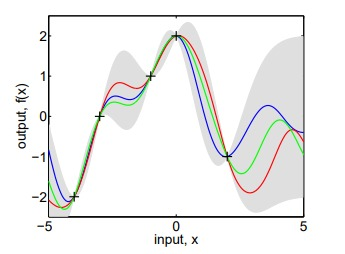
\includegraphics[width = 0.55\textwidth]{graph.jpeg}
    \caption{Graphical Representation}
\end{figure}


Here in this figure you can see that the points marked as + are the points in our dataset, for which the output is exactly one value while it is a distribution (as given by the shaded area) for all the other points (here assumed to be normal distribution).\\

Whenever we add an extra point to the dataset the mean line changes and passes through that point and the variance at that point becomes 0.\\

\subsection{Gaussian Process}
Gaussian processes are a method for non parametric estimation to provide confidence on the seen data and some kind of distribution on unseen data. For any subset of the training data, we must have that the joint prior distribution of this subset is normally distributed for some mean and covariance matrix.\\

For any subset $\{x_1 ... x_m\}$ of the training data, the prior distribution follows:

\[
\begin{bmatrix}
    f(x_1) \\
    \vdots \\
    f(x_m) \\
\end{bmatrix}
\quad \sim \quad
\mathcal{N} (\vec{\mu} (x_1,\dots ,x_m),\Sigma (x_1,\dots,x_m) )
\]
\\
where $\vec{\mu}$ and $\Sigma$ are deterministic functions.

As discussed earlier, On introducing a new data point into any subset of the training data, we expect the resulting conditional distribution to also follow the normal distribution. \\

For the data point $x^*$

\[
f(x^*) \vert (f(x_1), \dots f(x_m), x^*) \sim \mathcal{N}(\vec{\mu}(x_1,\dots,x_m,x^*), \Sigma(x_1,\dots,x_m,x^*))
\]

\subsection{Conditional Rule for Multi-variate Gaussian}

Intuitively, if we start with a Gaussian distribution and update our knowledge given the observed value of one of its components(that is, find conditional probability distribution), then the resulting distribution is still Gaussian! Mathematically,\\
Let $[x \text{ }y]$ jointly form multi variate Gaussian random variable,
\[
\begin{bmatrix}
    x \\
    y \\
\end{bmatrix} \sim
\mathcal{N}
\left(
\begin{bmatrix}
    \mu_x \\
    \mu_y \\
\end{bmatrix},
\begin{bmatrix}
    \Sigma_{xx} & \Sigma_{xy}\\
    \Sigma_{yx} & \Sigma_{yy}\\
\end{bmatrix}
\right)
\]

Here $\Sigma_{ab}$ represents covariance matrix between random vectors $a$ and $b$ and $f(\cdot)$ represents the PDF.

\[f(x\vert y) = \frac{f(x,y)}{f(y)}\]
Now, we will substitute $f(x,y)$ with the expression for multi-variate Gaussian distribution($\mathcal{N}(\mu, \Sigma)$), and $f(y)$ with $\mathcal{N}(\mu_{y}, \Sigma_{yy})$. 
Simplifying the equations, we get
\[
f(x\vert y)=
\mathcal{N}
(\Sigma_{xy}\Sigma_{yy}^{-1}y,
\Sigma_{xx} - \Sigma_{xy}\Sigma_{yy}^{-1}\Sigma_{yx})
\]
($\mu$ is assumed to be zero for simplicity)\\

\subsection{Updating Parameters on New data}
Suppose we have a training set \{y,x\} and a test set and we try to fit a model through it. Under what conditions will the model go through all the points? Fitting a higher order model would ensure high accuracy on the training set, but test set accuracy must be satisfied.\\

\noindent Given P(y|x) $\Rightarrow$ As long as we observe y, it's variance should go to zero.

\[P(y|x) = \mathcal{N}(\mu, \Sigma)\]
but if (x,y) $\in \{(x_i, y_i)\}_{i=1}^N$ then $\sigma = 0$
There can be error on points we don't observe, but there mustn't be error on already observed points.

\noindent To achieve this $\Rightarrow \underset{w}{min} \Sigma (y_i - w^Tx_i)^2 \rightarrow 0 $ where $x_i \rightarrow \phi(x_i)$ which dimension may tend to $\infty $.

$\phi(x_i)$ can't be finite as then it won't work for arbitrary number of training set. $w$ and $\phi(x)$ is not computable but $f(x_i) = \Sigma \alpha_i k (x,x_i) y_i$.
\[\underset{\alpha}{min} \Sigma (y_i - \alpha_i k (x, x_i) y_i\]
\[\underset{\alpha}{min} \sum_{j} \left[\sum_{i} y_i - \alpha_i k (x, x_i) y_i ) \right]^2 \]
If we observe new point $y_i$, we have to adjust $\alpha_i$ such that to keep variance = 0.

% \bibliographystyle{abbrv}           % if you need a bibliography
% \bibliography{mybib}                % assuming yours is named mybib.bib


\end{document}
